\documentclass[a4paper,12pt]{article} 

% First, we usually want to set the margins of our document. For this we use the package geometry.
\usepackage[top = 2.5cm, bottom = 2.5cm, left = 2.5cm, right = 2.5cm]{geometry} 
\usepackage[T1]{fontenc}
\usepackage[utf8]{inputenc}

% The following two packages - multirow and booktabs - are needed to create nice looking tables.
\usepackage{multirow} % Multirow is for tables with multiple rows within one cell.
\usepackage{booktabs} % For even nicer tables.

% As we usually want to include some plots (.pdf files) we need a package for that.
\usepackage{graphicx} 

% The default setting of LaTeX is to indent new paragraphs. This is useful for articles. But not really nice for homework problem sets. The following command sets the indent to 0.
% \usepackage{setspace}
% \setlength{\parindent}{0in}
\usepackage{indentfirst}

% Package to place figures where you want them.
\usepackage{float}

% The fancyhdr package let's us create nice headers.
\usepackage{fancyhdr}

\usepackage{xcolor,amsmath,amsthm,algorithm2e,tikz,subcaption}
\RestyleAlgo{ruled}

\definecolor{myRed}{RGB}{211, 31, 17}
\definecolor{myOrange}{RGB}{244, 122, 0}
\definecolor{myLightTeal}{RGB}{98, 200, 211}
\definecolor{myDarkTeal}{RGB}{0, 113, 145}


% To make our document nice we want a header and number the pages in the footer.

\pagestyle{fancy} % With this command we can customize the header style.

\fancyhf{} % This makes sure we do not have other information in our header or footer.

\lhead{\footnotesize Algorithm Design and Analysis(H): Assignment 6}% \lhead puts text in the top left corner. \footnotesize sets our font to a smaller size.

%\rhead works just like \lhead (you can also use \chead)
\rhead{\footnotesize Mengxuan Wu} %<---- Fill in your lastnames.

% Similar commands work for the footer (\lfoot, \cfoot and \rfoot).
% We want to put our page number in the center.
\cfoot{\footnotesize \thepage} 

\begin{document}

\thispagestyle{empty} % This command disables the header on the first page. 

\begin{tabular}{p{15.5cm}}
{\large \bf Algorithm Design and Analysis(H)} \\
Southern University of Science and Technology \\ Mengxuan Wu \\ 12212006 \\
\hline
\\
\end{tabular}

\begin{center}
	{\Large \bf Assignment 6 \\ NP-Completeness}
	\vspace{2mm}

	{\bf Polynomial-time Reduction from 3-SAT to 3-Coloring}
	\vspace{2mm}

	{\bf Mengxuan Wu}
		
\end{center}

\section{3-Coloring}

\subsection{Problem Definition}

Given an undirected graph $G = (V, E)$, a coloring of $G$ is an assignment of colors to the vertices of $G$ such that no two adjacent vertices have the same color. 
The 3-coloring problem is to determine whether a given graph $G$ can be colored with at most 3 colors.

\subsection{Proof of NP}

A certificate for the 3-coloring problem is an assignment of colors to the vertices of $G$. 
We can verify this certificate in polynomial time by:
\begin{enumerate}
	\item Checking each edge in $E$ to ensure no two adjacent vertices have the same color, which takes $O(|E|) = O(|V|^2)$ time.
	\item Counting the number of colors used in the certificate, which takes $O(|V|)$ time.
\end{enumerate}

Thus, the verification algorithm runs in polynomial time, so the 3-coloring problem is in NP.

\section{Polynomial-time Reduction from 3-SAT to 3-Coloring}

\subsection{Base Graph Construction}

We first construct a base graph $G_{\text{base}}$ with 3 initial vertices: Base, True, and False, which are connected in a cycle.
Then for each variable $v_i$ in the 3-SAT formula, we add two vertices $v_i$ and $\overline{v_i}$ to $G_{\text{base}}$.
We join each pair of $v_i$ and $\overline{v_i}$ together and connect them to the Base vertex, which will form a triangle with the Base vertex, $v_i$, and $\overline{v_i}$.

An example of the base graph with 3 variables is shown in Figure \ref{fig:base}.
\begin{figure}[H]
	\centering
	\begin{tikzpicture}
		\draw (0, -2.6) 	node[draw, circle, minimum size=1.5cm] (base) 	{Base};
		\draw (1.5, 0) 		node[draw, circle, minimum size=1.5cm] (false) 	{False};
		\draw (-1.5, 0) 	node[draw, circle, minimum size=1.5cm] (true) 	{True};
		\draw (-6, -6)      node[draw, circle, minimum size=1.5cm] (v1) 	{$v_1$};
		\draw (-4, -6)      node[draw, circle, minimum size=1.5cm] (v1') 	{$\overline{v_1}$};
		\draw (-1, -7)	  	node[draw, circle, minimum size=1.5cm] (v2) 	{$v_2$};
		\draw (1, -7)	  	node[draw, circle, minimum size=1.5cm] (v2') 	{$\overline{v_2}$};
		\draw (4, -6)	  	node[draw, circle, minimum size=1.5cm] (v3) 	{$v_3$};
		\draw (6, -6)	  	node[draw, circle, minimum size=1.5cm] (v3') 	{$\overline{v_3}$};

		\draw (base) -- (false) -- (true) -- (base);
		\draw (base) -- (v1) -- (v1') -- (base);
		\draw (base) -- (v2) -- (v2') -- (base);
		\draw (base) -- (v3) -- (v3') -- (base);
	\end{tikzpicture}
	\caption{Base Graph $G_{\text{base}}$ with 3 Variables}
	\label{fig:base}
\end{figure}

We can notice that the base graph $G_{\text{base}}$ already obtains some important properties:
\begin{enumerate}
	\item The graph can be 3-colored.
	\item The True, False, and Base vertices will be colored with 3 different colors.
	\item For all the variable vertices $v_i$ and $\overline{v_i}$, one of them will be colored with the same color as the True vertex, and the other will be colored with the same color as the False vertex.
\end{enumerate}

For the sake of simplicity, we call the color of the True vertex as True color, the color of the False vertex as False color, and the color of the Base vertex as Base color.
For all the variable vertices $v_i$ colored with the True color, we assign the value of $v_i$ to be True.
And for all the variable vertices $v_i$ colored with the False color, we assign the value of $v_i$ to be False.

We can observe that the properties of the base graph $G_{\text{base}}$ help us maintain the consistency of the variable values.
It guarantees that if $v_i$ is True, then $\overline{v_i}$ must be False, and vice versa.
Also, it ensures that each variable $v_i$ will be assigned with either True or False.

\subsection{Clause Graph Construction}

With the base graph $G_{\text{base}}$ constructed, we can now build the clause graph $G_{\text{clause}}$ for each clause in the 3-SAT formula.
For each clause $C_j = v_1 \vee v_2 \vee v_3$, we build a subgraph $G_{\text{clause}}^j$ as shown in Figure \ref{fig:clause}.

\begin{figure}[H]
	\centering
	\resizebox{0.7\linewidth}{!}{
		\begin{tikzpicture}
			\draw (0, 0) 	node[draw, circle, minimum size=1.5cm] 	(v1) 		{$v_1$};
			\draw (5, 0) 	node[draw, circle, minimum size=1.5cm] 	(true) 		{True};
			\draw (10, 0) 	node[draw, circle, minimum size=1.5cm] 	(v3) 		{$v_3$};
			\draw (15, 0) 	node[draw, circle, minimum size=1.5cm] 	(false) 	{False};
			\draw (0, 3) 	node[draw, circle, minimum size=1.5cm] 	(v1_a) 		{};
			\draw (7.5, 4) 	node[draw, circle, minimum size=1.5cm] 	(v2) 		{$v_2$};
			\draw (10, 3) 	node[draw, circle, minimum size=1.5cm] 	(v3_a) 		{};
			\draw (0, 6) 	node[draw, circle, minimum size=1.5cm] 	(v1_aa) 	{};
			\draw (5, 6) 	node[draw, circle, minimum size=1.5cm] 	(v2_aa) 	{};
			\draw (10, 6) 	node[draw, circle, minimum size=1.5cm] 	(v3_aa) 	{};
			\draw (5, 9) 	node[draw, circle, minimum size=1.5cm] 	(top) 		{};
	
			\draw (v1) -- (v1_a) -- (v1_aa) -- (top);
			\draw (v2) -- (v2_aa) -- (top);
			\draw (v3) -- (v3_a) -- (v3_aa) -- (top);
			\draw (true) -- (v1_a);
			\draw (true) -- (v1_aa);
			\draw (true) -- (v2_aa);
			\draw (true) -- (v3_a);
			\draw (false) -- (v3_aa);
		\end{tikzpicture}
	}
	\caption{Clause Graph $G_{\text{clause}}^j$ for Clause $C_j = v_1 \vee v_2 \vee v_3$}
	\label{fig:clause}
\end{figure}

The clause graph $G_{\text{clause}}$ has the property that if and only if all the variable vertices are colored with the False color, then there does not exist a 3-coloring for the clause graph.

\begin{proof}
$ $	

\paragraph{\textbf{If} part}

\begin{figure}[H]
	\centering
	\resizebox{0.7\linewidth}{!}{
		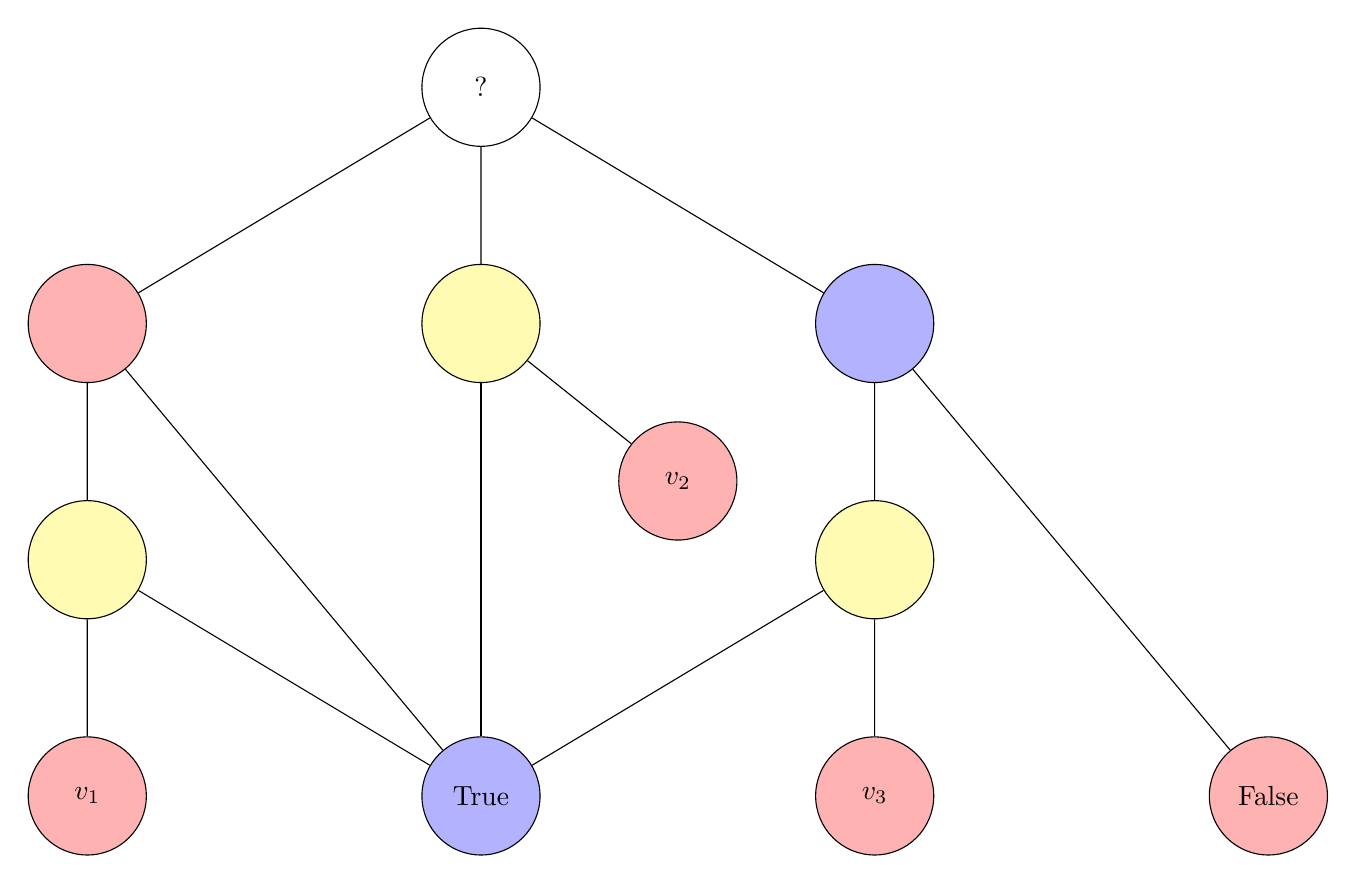
\begin{tikzpicture}
			\draw (0, 0) 	node[draw, circle, minimum size=1.5cm, fill=red!30] 	(v1) 		{$v_1$};
			\draw (5, 0) 	node[draw, circle, minimum size=1.5cm, fill=blue!30] 	(true) 		{True};
			\draw (10, 0) 	node[draw, circle, minimum size=1.5cm, fill=red!30] 	(v3) 		{$v_3$};
			\draw (15, 0) 	node[draw, circle, minimum size=1.5cm, fill=red!30] 	(false) 	{False};
			\draw (0, 3) 	node[draw, circle, minimum size=1.5cm, fill=yellow!30] 	(v1_a) 		{};
			\draw (7.5, 4) 	node[draw, circle, minimum size=1.5cm, fill=red!30] 	(v2) 		{$v_2$};
			\draw (10, 3) 	node[draw, circle, minimum size=1.5cm, fill=yellow!30] 	(v3_a) 		{};
			\draw (0, 6) 	node[draw, circle, minimum size=1.5cm, fill=red!30] 	(v1_aa) 	{};
			\draw (5, 6) 	node[draw, circle, minimum size=1.5cm, fill=yellow!30] 	(v2_aa) 	{};
			\draw (10, 6) 	node[draw, circle, minimum size=1.5cm, fill=blue!30] 	(v3_aa) 	{};
			\draw (5, 9) 	node[draw, circle, minimum size=1.5cm] 					(top) 		{?};
	
			\draw (v1) -- (v1_a) -- (v1_aa) -- (top);
			\draw (v2) -- (v2_aa) -- (top);
			\draw (v3) -- (v3_a) -- (v3_aa) -- (top);
			\draw (true) -- (v1_a);
			\draw (true) -- (v1_aa);
			\draw (true) -- (v2_aa);
			\draw (true) -- (v3_a);
			\draw (false) -- (v3_aa);
		\end{tikzpicture}
	}
	\caption{Clause Graph $G_{\text{clause}}^j$ with All Variable Vertices Colored with the False Color}
	\label{fig:clause_false}
\end{figure}

An example of all the variable vertices colored with the False color is shown in Figure \ref{fig:clause_false}.
We first give the variable vertices the False color, and color the True and False vertices with the True and False colors, respectively.
The remaining part of the graph must be colored in this specific way. 
This is because the colored vertices constrain their neighboring vertices to pick the single remaining available colors, effectively determining the coloring for the rest of the graph.

As we can see, the top vertex in the clause graph $G_{\text{clause}}^j$ cannot be colored with any of the 3 colors, since the second layer of vertices it connects to are colored with all 3 colors.
This means for a clause graph $G_{\text{clause}}^j$, if all the variable vertices are colored with the False color, then there does not exist a 3-coloring for the clause graph.

\paragraph{\textbf{Only If} part}

If any of the variable vertices are colored with the True color, then there exists a 3-coloring for the clause graph.
For the sake of simplicity here, we put the coloring of the clause graph for all other possible variable values in appendix \ref{app:clause}.
\end{proof}

\subsection{Final Graph Construction}

The final graph $G_{\text{final}}$ is constructed by:
\begin{enumerate}
	\item Constructing the base graph $G_{\text{base}}$.
	\item For each clause $C_j = v_1 \vee v_2 \vee v_3$, constructing the clause graph $G_{\text{clause}}^j$ and merge it with the base graph $G_{\text{base}}$.
\end{enumerate}

The 3-SAT formula is satisfiable if and only if there exists a 3-coloring for the corresponding final graph $G_{\text{final}}$.

\begin{proof}
$ $

\paragraph{\textbf{If} part}

If the 3-SAT formula is satisfiable, then there exists a truth assignment that satisfies all the clauses.
We can assign the True color to the True vertex and the False color to the False vertex in the final graph $G_{\text{final}}$.
Since each clause is satisfied, there exists some 3-color assignment for each clause graph as well.
Thus, there exists a 3-coloring for the final graph $G_{\text{final}}$.

\paragraph{\textbf{Only If} part}
If there exists a 3-coloring for the final graph $G_{\text{final}}$, then we assign variable values based on the coloring of the variable vertices in the final graph.
Since each clause graph has a 3-coloring, the corresponding clause is satisfied.
Thus, the 3-SAT formula is satisfiable.
\end{proof}

Hence, for each 3-SAT formula, we can construct a corresponding final graph $G_{\text{final}}$.
If we can determine whether there exists a 3-coloring for the final graph $G_{\text{final}}$, then we can solve the 3-SAT problem.
Thus, the 3-SAT problem is polynomial-time reducible to the 3-coloring problem.

\newpage

\appendix

\section{Clause Graph Coloring}
\label{app:clause}

\textit{Some graph may have multiple 3-colorings. Here we only show one of the possible 3-colorings for each clause graph.}

\begin{figure}[H]
	\centering
	\resizebox{0.6\linewidth}{!}{
		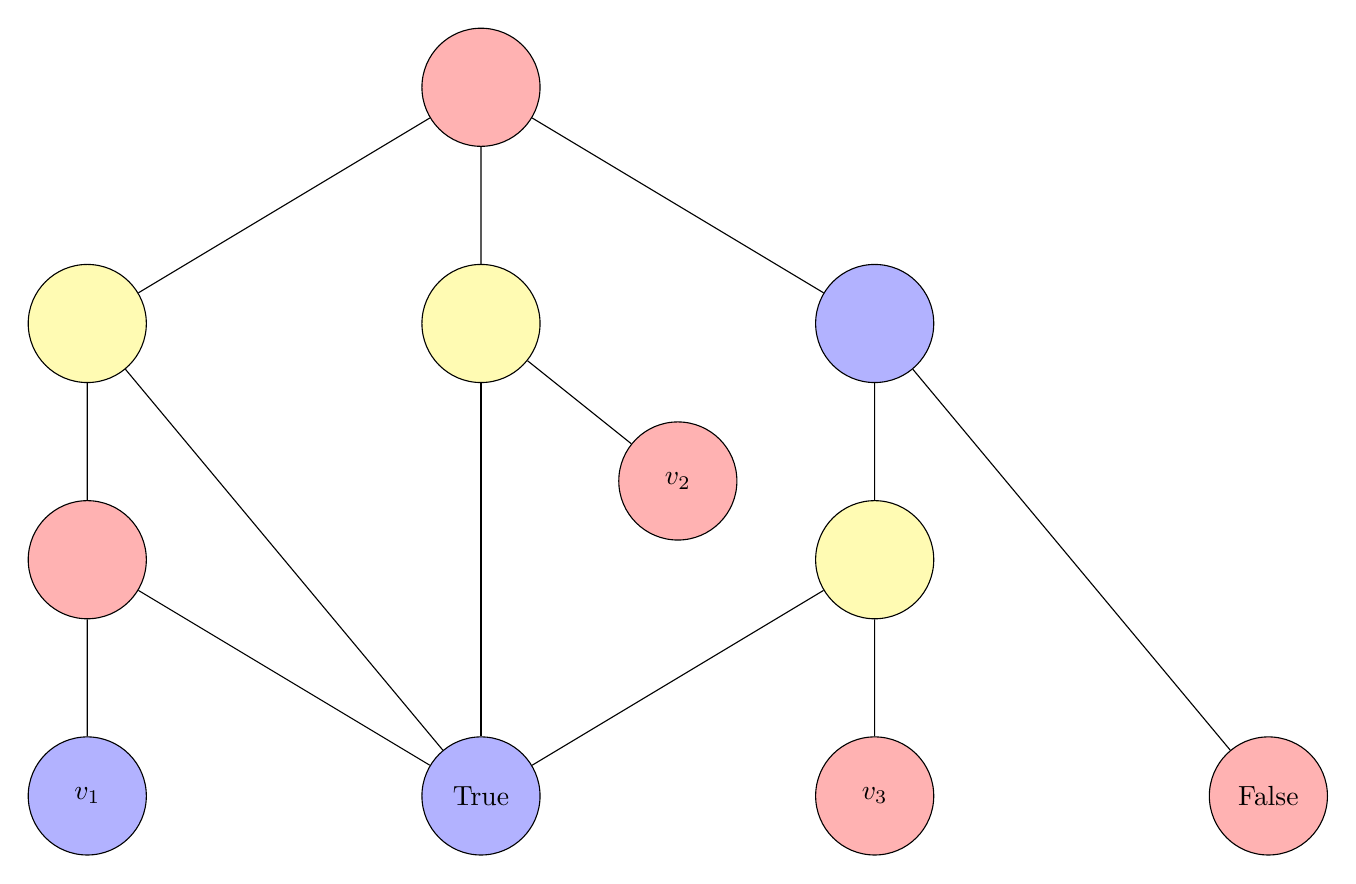
\begin{tikzpicture}
			\draw (0, 0) 	node[draw, circle, minimum size=1.5cm, fill=blue!30] 	(v1) 		{$v_1$};
			\draw (5, 0) 	node[draw, circle, minimum size=1.5cm, fill=blue!30] 	(true) 		{True};
			\draw (10, 0) 	node[draw, circle, minimum size=1.5cm, fill=red!30] 	(v3) 		{$v_3$};
			\draw (15, 0) 	node[draw, circle, minimum size=1.5cm, fill=red!30] 	(false) 	{False};
			\draw (0, 3) 	node[draw, circle, minimum size=1.5cm, fill=red!30] 	(v1_a) 		{};
			\draw (7.5, 4) 	node[draw, circle, minimum size=1.5cm, fill=red!30] 	(v2) 		{$v_2$};
			\draw (10, 3) 	node[draw, circle, minimum size=1.5cm, fill=yellow!30] 	(v3_a) 		{};
			\draw (0, 6) 	node[draw, circle, minimum size=1.5cm, fill=yellow!30] 	(v1_aa) 	{};
			\draw (5, 6) 	node[draw, circle, minimum size=1.5cm, fill=yellow!30] 	(v2_aa) 	{};
			\draw (10, 6) 	node[draw, circle, minimum size=1.5cm, fill=blue!30] 	(v3_aa) 	{};
			\draw (5, 9) 	node[draw, circle, minimum size=1.5cm, fill=red!30] 	(top) 		{};
	
			\draw (v1) -- (v1_a) -- (v1_aa) -- (top);
			\draw (v2) -- (v2_aa) -- (top);
			\draw (v3) -- (v3_a) -- (v3_aa) -- (top);
			\draw (true) -- (v1_a);
			\draw (true) -- (v1_aa);
			\draw (true) -- (v2_aa);
			\draw (true) -- (v3_a);
			\draw (false) -- (v3_aa);
		\end{tikzpicture}
	}
	\caption{Clause Graph $G_{\text{clause}}^j$ with $v_1 = \text{True}$, $v_2 = \text{False}$, and $v_3 = \text{False}$}
\end{figure}

\begin{figure}[H]
	\centering
	\resizebox{0.6\linewidth}{!}{
		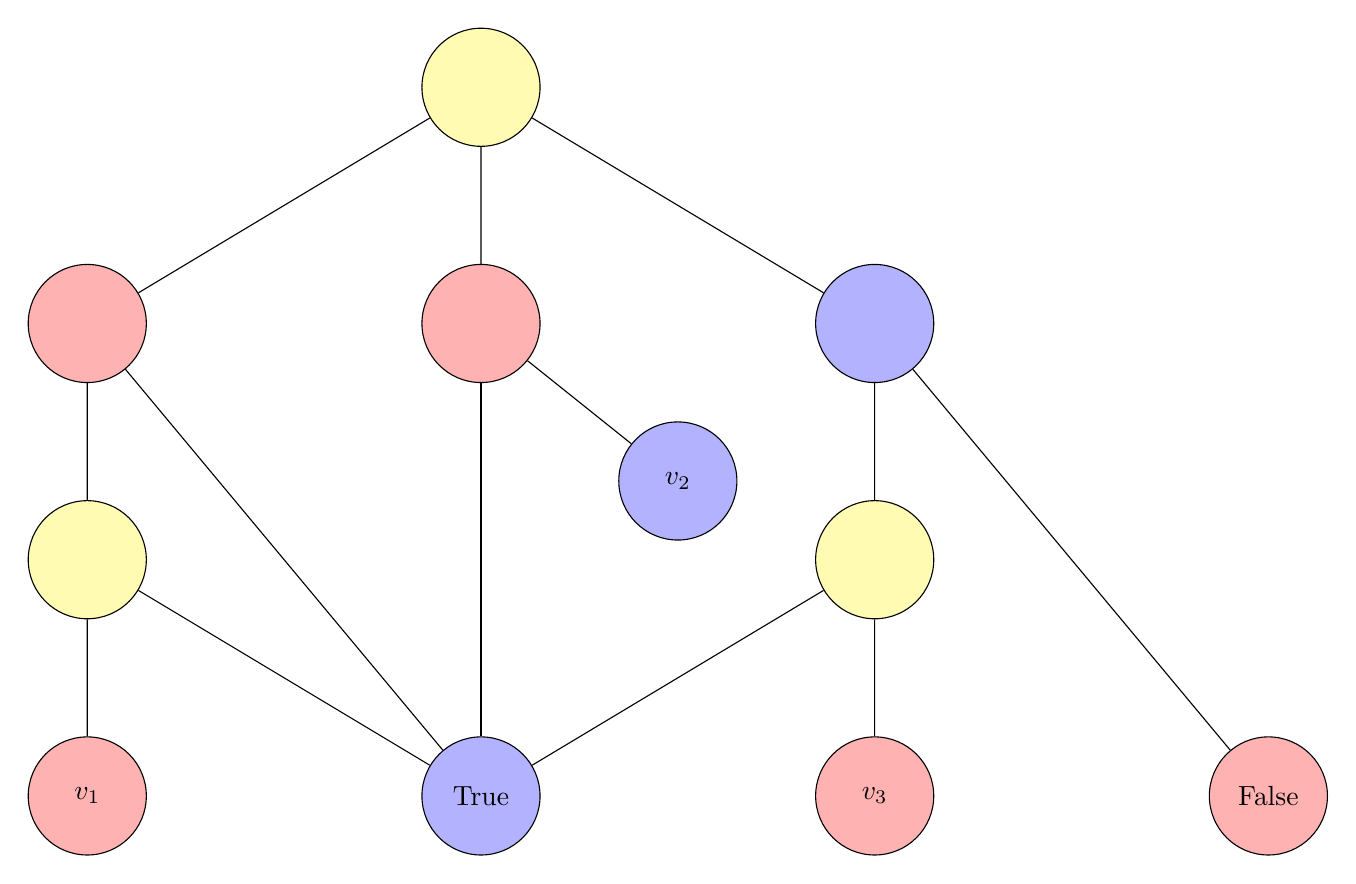
\begin{tikzpicture}
			\draw (0, 0) 	node[draw, circle, minimum size=1.5cm, fill=red!30] 	(v1) 		{$v_1$};
			\draw (5, 0) 	node[draw, circle, minimum size=1.5cm, fill=blue!30] 	(true) 		{True};
			\draw (10, 0) 	node[draw, circle, minimum size=1.5cm, fill=red!30] 	(v3) 		{$v_3$};
			\draw (15, 0) 	node[draw, circle, minimum size=1.5cm, fill=red!30] 	(false) 	{False};
			\draw (0, 3) 	node[draw, circle, minimum size=1.5cm, fill=yellow!30] 	(v1_a) 		{};
			\draw (7.5, 4) 	node[draw, circle, minimum size=1.5cm, fill=blue!30] 	(v2) 		{$v_2$};
			\draw (10, 3) 	node[draw, circle, minimum size=1.5cm, fill=yellow!30] 	(v3_a) 		{};
			\draw (0, 6) 	node[draw, circle, minimum size=1.5cm, fill=red!30] 	(v1_aa) 	{};
			\draw (5, 6) 	node[draw, circle, minimum size=1.5cm, fill=red!30] 	(v2_aa) 	{};
			\draw (10, 6) 	node[draw, circle, minimum size=1.5cm, fill=blue!30] 	(v3_aa) 	{};
			\draw (5, 9) 	node[draw, circle, minimum size=1.5cm, fill=yellow!30] 	(top) 		{};
	
			\draw (v1) -- (v1_a) -- (v1_aa) -- (top);
			\draw (v2) -- (v2_aa) -- (top);
			\draw (v3) -- (v3_a) -- (v3_aa) -- (top);
			\draw (true) -- (v1_a);
			\draw (true) -- (v1_aa);
			\draw (true) -- (v2_aa);
			\draw (true) -- (v3_a);
			\draw (false) -- (v3_aa);
		\end{tikzpicture}
	}
	\caption{Clause Graph $G_{\text{clause}}^j$ with $v_1 = \text{False}$, $v_2 = \text{True}$, and $v_3 = \text{False}$}
\end{figure}

\begin{figure}[H]
	\centering
	\resizebox{0.6\linewidth}{!}{
		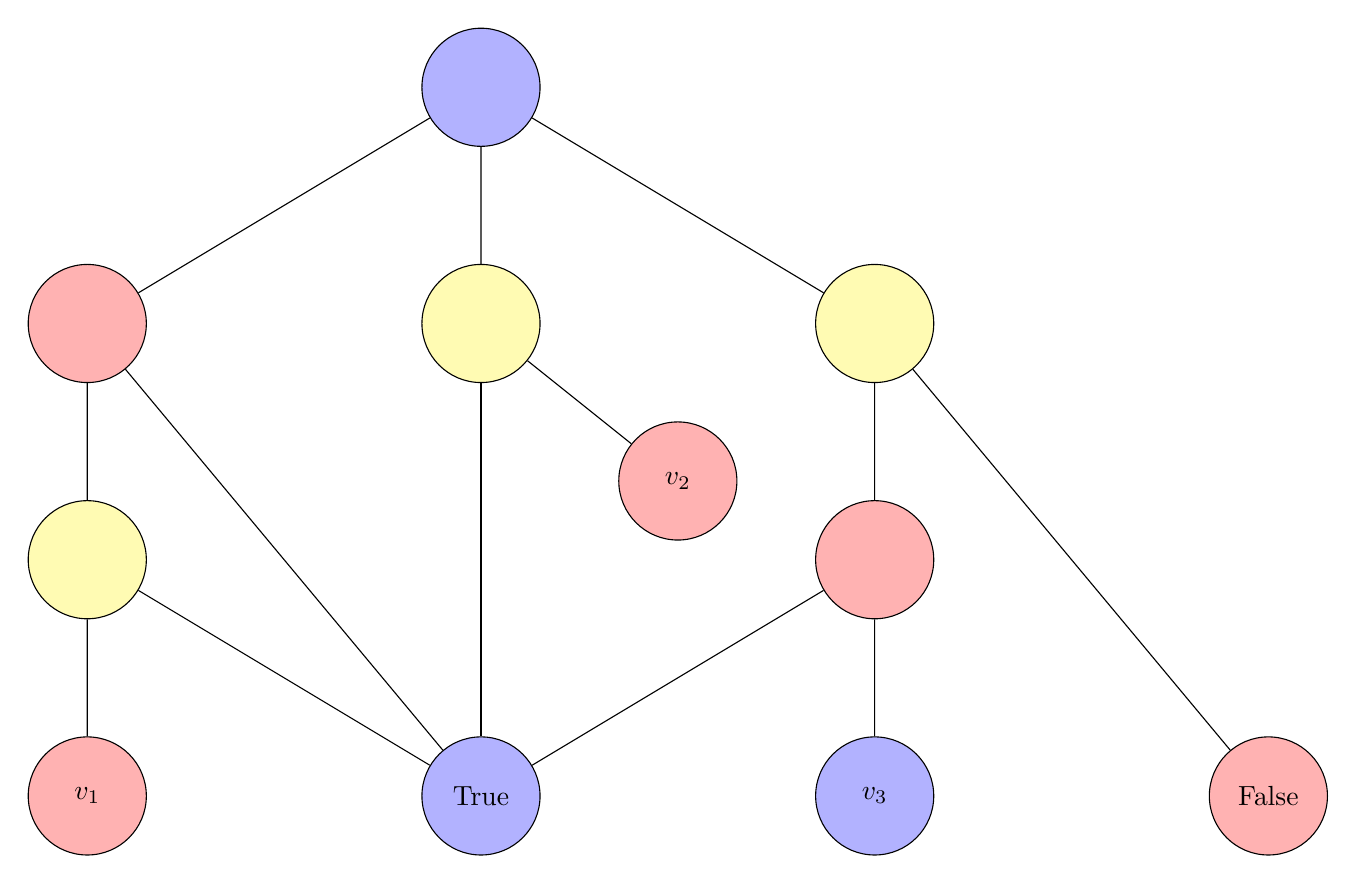
\begin{tikzpicture}
			\draw (0, 0) 	node[draw, circle, minimum size=1.5cm, fill=red!30] 	(v1) 		{$v_1$};
			\draw (5, 0) 	node[draw, circle, minimum size=1.5cm, fill=blue!30] 	(true) 		{True};
			\draw (10, 0) 	node[draw, circle, minimum size=1.5cm, fill=blue!30] 	(v3) 		{$v_3$};
			\draw (15, 0) 	node[draw, circle, minimum size=1.5cm, fill=red!30] 	(false) 	{False};
			\draw (0, 3) 	node[draw, circle, minimum size=1.5cm, fill=yellow!30] 	(v1_a) 		{};
			\draw (7.5, 4) 	node[draw, circle, minimum size=1.5cm, fill=red!30] 	(v2) 		{$v_2$};
			\draw (10, 3) 	node[draw, circle, minimum size=1.5cm, fill=red!30] 	(v3_a) 		{};
			\draw (0, 6) 	node[draw, circle, minimum size=1.5cm, fill=red!30] 	(v1_aa) 	{};
			\draw (5, 6) 	node[draw, circle, minimum size=1.5cm, fill=yellow!30] 	(v2_aa) 	{};
			\draw (10, 6) 	node[draw, circle, minimum size=1.5cm, fill=yellow!30] 	(v3_aa) 	{};
			\draw (5, 9) 	node[draw, circle, minimum size=1.5cm, fill=blue!30] 	(top) 		{};
	
			\draw (v1) -- (v1_a) -- (v1_aa) -- (top);
			\draw (v2) -- (v2_aa) -- (top);
			\draw (v3) -- (v3_a) -- (v3_aa) -- (top);
			\draw (true) -- (v1_a);
			\draw (true) -- (v1_aa);
			\draw (true) -- (v2_aa);
			\draw (true) -- (v3_a);
			\draw (false) -- (v3_aa);
		\end{tikzpicture}
	}
	\caption{Clause Graph $G_{\text{clause}}^j$ with $v_1 = \text{False}$, $v_2 = \text{False}$, and $v_3 = \text{True}$}
\end{figure}

\begin{figure}[H]
	\centering
	\resizebox{0.6\linewidth}{!}{
		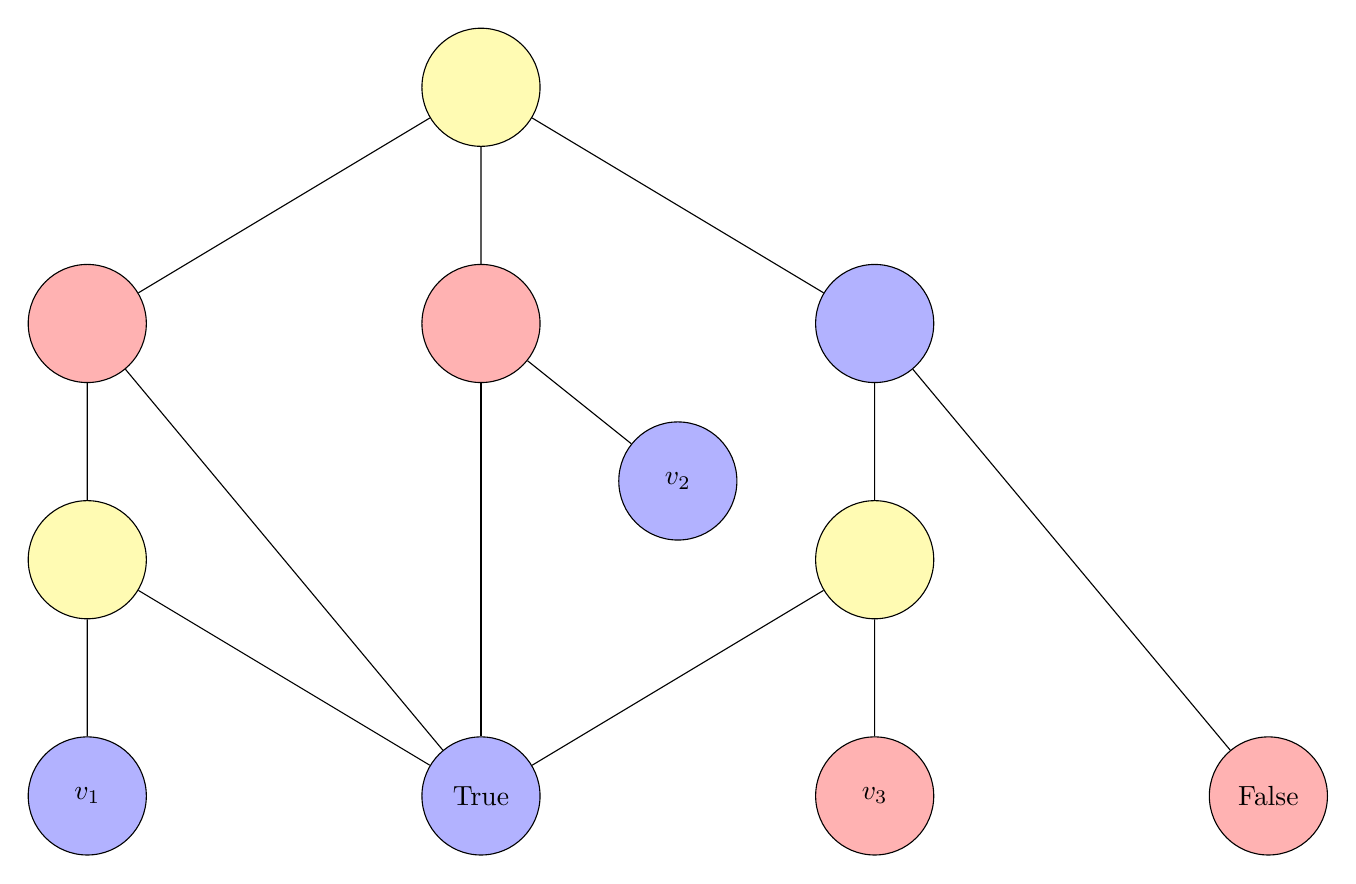
\begin{tikzpicture}
			\draw (0, 0) 	node[draw, circle, minimum size=1.5cm, fill=blue!30] 	(v1) 		{$v_1$};
			\draw (5, 0) 	node[draw, circle, minimum size=1.5cm, fill=blue!30] 	(true) 		{True};
			\draw (10, 0) 	node[draw, circle, minimum size=1.5cm, fill=red!30] 	(v3) 		{$v_3$};
			\draw (15, 0) 	node[draw, circle, minimum size=1.5cm, fill=red!30] 	(false) 	{False};
			\draw (0, 3) 	node[draw, circle, minimum size=1.5cm, fill=yellow!30] 	(v1_a) 		{};
			\draw (7.5, 4) 	node[draw, circle, minimum size=1.5cm, fill=blue!30] 	(v2) 		{$v_2$};
			\draw (10, 3) 	node[draw, circle, minimum size=1.5cm, fill=yellow!30] 	(v3_a) 		{};
			\draw (0, 6) 	node[draw, circle, minimum size=1.5cm, fill=red!30] 	(v1_aa) 	{};
			\draw (5, 6) 	node[draw, circle, minimum size=1.5cm, fill=red!30] 	(v2_aa) 	{};
			\draw (10, 6) 	node[draw, circle, minimum size=1.5cm, fill=blue!30] 	(v3_aa) 	{};
			\draw (5, 9) 	node[draw, circle, minimum size=1.5cm, fill=yellow!30] 	(top) 		{};
	
			\draw (v1) -- (v1_a) -- (v1_aa) -- (top);
			\draw (v2) -- (v2_aa) -- (top);
			\draw (v3) -- (v3_a) -- (v3_aa) -- (top);
			\draw (true) -- (v1_a);
			\draw (true) -- (v1_aa);
			\draw (true) -- (v2_aa);
			\draw (true) -- (v3_a);
			\draw (false) -- (v3_aa);
		\end{tikzpicture}
	}
	\caption{Clause Graph $G_{\text{clause}}^j$ with $v_1 = \text{True}$, $v_2 = \text{True}$, and $v_3 = \text{False}$}
\end{figure}

\begin{figure}[H]
	\centering
	\resizebox{0.6\linewidth}{!}{
		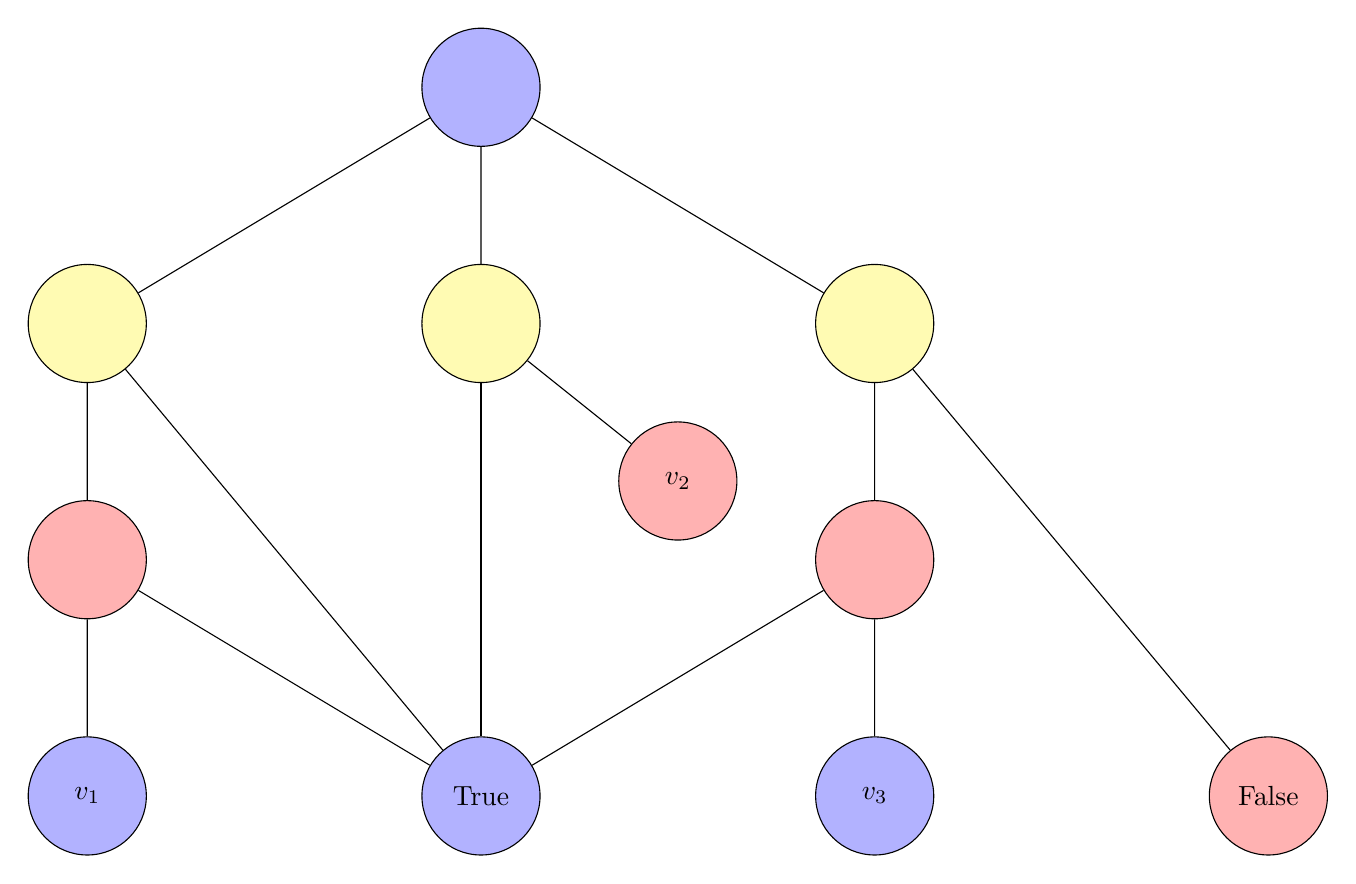
\begin{tikzpicture}
			\draw (0, 0) 	node[draw, circle, minimum size=1.5cm, fill=blue!30] 	(v1) 		{$v_1$};
			\draw (5, 0) 	node[draw, circle, minimum size=1.5cm, fill=blue!30] 	(true) 		{True};
			\draw (10, 0) 	node[draw, circle, minimum size=1.5cm, fill=blue!30] 	(v3) 		{$v_3$};
			\draw (15, 0) 	node[draw, circle, minimum size=1.5cm, fill=red!30] 	(false) 	{False};
			\draw (0, 3) 	node[draw, circle, minimum size=1.5cm, fill=red!30] 	(v1_a) 		{};
			\draw (7.5, 4) 	node[draw, circle, minimum size=1.5cm, fill=red!30] 	(v2) 		{$v_2$};
			\draw (10, 3) 	node[draw, circle, minimum size=1.5cm, fill=red!30] 	(v3_a) 		{};
			\draw (0, 6) 	node[draw, circle, minimum size=1.5cm, fill=yellow!30] 	(v1_aa) 	{};
			\draw (5, 6) 	node[draw, circle, minimum size=1.5cm, fill=yellow!30] 	(v2_aa) 	{};
			\draw (10, 6) 	node[draw, circle, minimum size=1.5cm, fill=yellow!30] 	(v3_aa) 	{};
			\draw (5, 9) 	node[draw, circle, minimum size=1.5cm, fill=blue!30] 	(top) 		{};
	
			\draw (v1) -- (v1_a) -- (v1_aa) -- (top);
			\draw (v2) -- (v2_aa) -- (top);
			\draw (v3) -- (v3_a) -- (v3_aa) -- (top);
			\draw (true) -- (v1_a);
			\draw (true) -- (v1_aa);
			\draw (true) -- (v2_aa);
			\draw (true) -- (v3_a);
			\draw (false) -- (v3_aa);
		\end{tikzpicture}
	}
	\caption{Clause Graph $G_{\text{clause}}^j$ with $v_1 = \text{True}$, $v_2 = \text{False}$, and $v_3 = \text{True}$}
\end{figure}

\begin{figure}[H]
	\centering
	\resizebox{0.6\linewidth}{!}{
		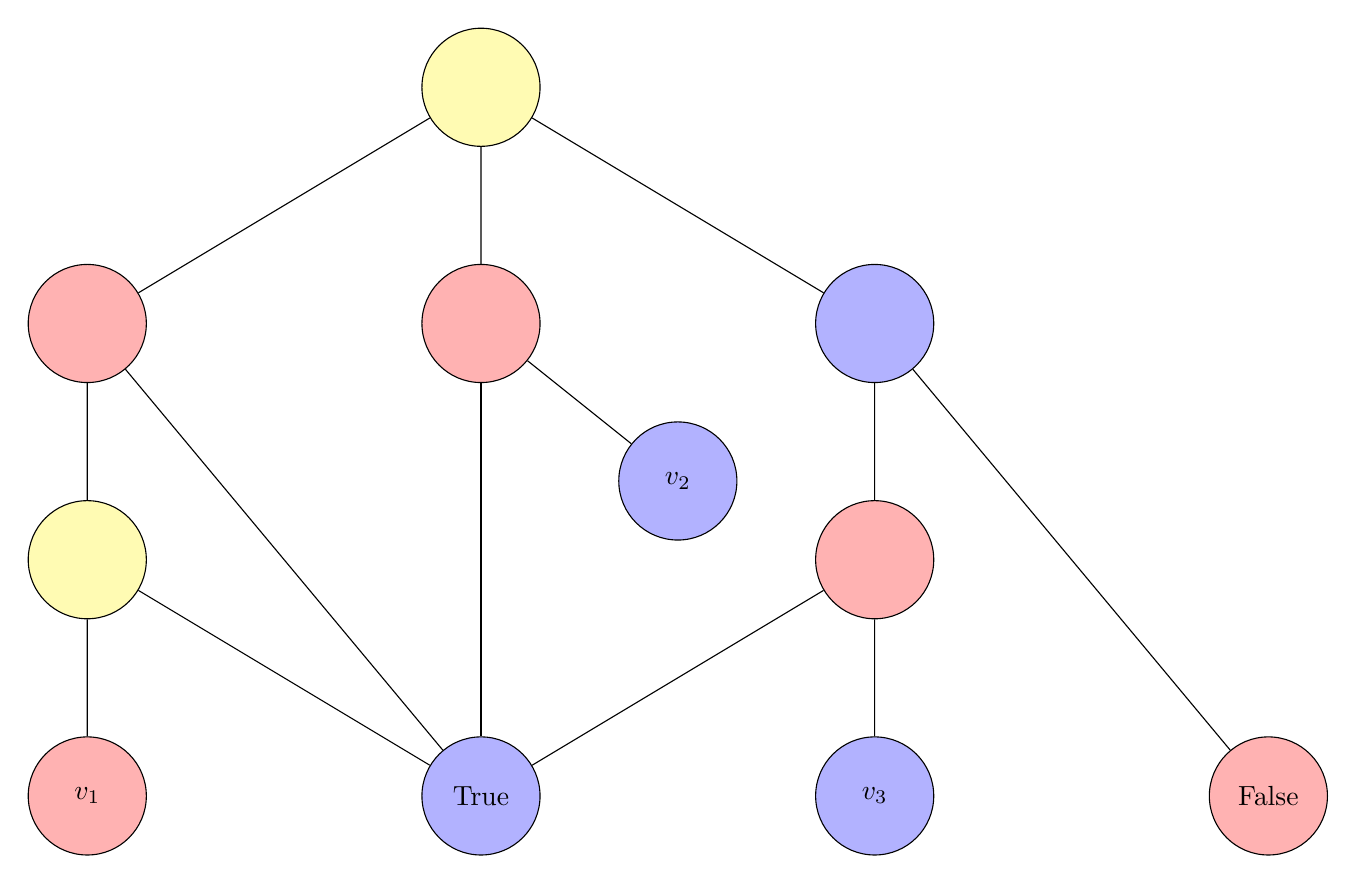
\begin{tikzpicture}
			\draw (0, 0) 	node[draw, circle, minimum size=1.5cm, fill=red!30] 	(v1) 		{$v_1$};
			\draw (5, 0) 	node[draw, circle, minimum size=1.5cm, fill=blue!30] 	(true) 		{True};
			\draw (10, 0) 	node[draw, circle, minimum size=1.5cm, fill=blue!30] 	(v3) 		{$v_3$};
			\draw (15, 0) 	node[draw, circle, minimum size=1.5cm, fill=red!30] 	(false) 	{False};
			\draw (0, 3) 	node[draw, circle, minimum size=1.5cm, fill=yellow!30] 	(v1_a) 		{};
			\draw (7.5, 4) 	node[draw, circle, minimum size=1.5cm, fill=blue!30] 	(v2) 		{$v_2$};
			\draw (10, 3) 	node[draw, circle, minimum size=1.5cm, fill=red!30] 	(v3_a) 		{};
			\draw (0, 6) 	node[draw, circle, minimum size=1.5cm, fill=red!30] 	(v1_aa) 	{};
			\draw (5, 6) 	node[draw, circle, minimum size=1.5cm, fill=red!30] 	(v2_aa) 	{};
			\draw (10, 6) 	node[draw, circle, minimum size=1.5cm, fill=blue!30] 	(v3_aa) 	{};
			\draw (5, 9) 	node[draw, circle, minimum size=1.5cm, fill=yellow!30] 	(top) 		{};
	
			\draw (v1) -- (v1_a) -- (v1_aa) -- (top);
			\draw (v2) -- (v2_aa) -- (top);
			\draw (v3) -- (v3_a) -- (v3_aa) -- (top);
			\draw (true) -- (v1_a);
			\draw (true) -- (v1_aa);
			\draw (true) -- (v2_aa);
			\draw (true) -- (v3_a);
			\draw (false) -- (v3_aa);
		\end{tikzpicture}
	}
	\caption{Clause Graph $G_{\text{clause}}^j$ with $v_1 = \text{False}$, $v_2 = \text{True}$, and $v_3 = \text{True}$}
\end{figure}

\begin{figure}[H]
	\centering
	\resizebox{0.6\linewidth}{!}{
		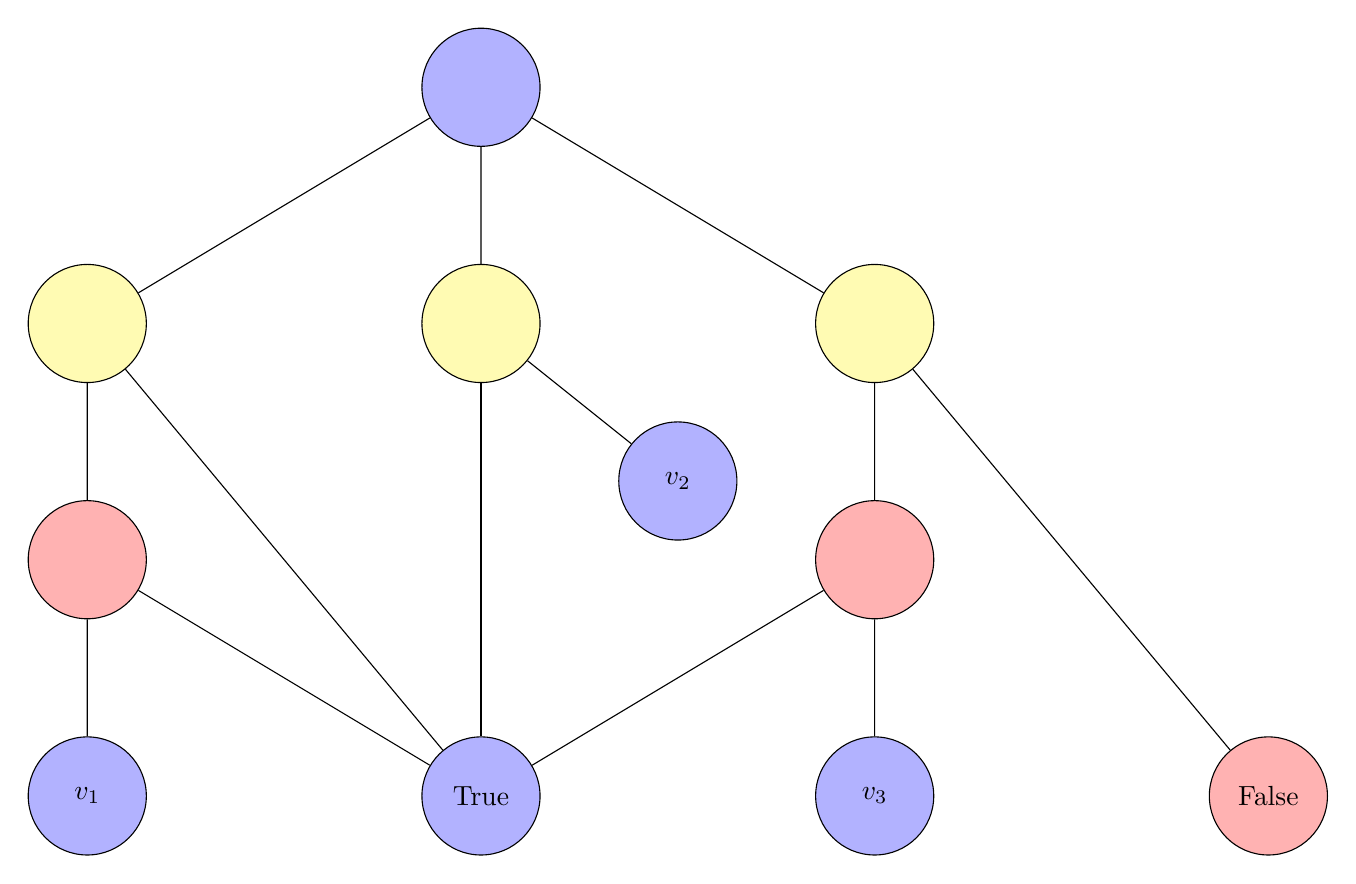
\begin{tikzpicture}
			\draw (0, 0) 	node[draw, circle, minimum size=1.5cm, fill=blue!30] 	(v1) 		{$v_1$};
			\draw (5, 0) 	node[draw, circle, minimum size=1.5cm, fill=blue!30] 	(true) 		{True};
			\draw (10, 0) 	node[draw, circle, minimum size=1.5cm, fill=blue!30] 	(v3) 		{$v_3$};
			\draw (15, 0) 	node[draw, circle, minimum size=1.5cm, fill=red!30] 	(false) 	{False};
			\draw (0, 3) 	node[draw, circle, minimum size=1.5cm, fill=red!30] 	(v1_a) 		{};
			\draw (7.5, 4) 	node[draw, circle, minimum size=1.5cm, fill=blue!30] 	(v2) 		{$v_2$};
			\draw (10, 3) 	node[draw, circle, minimum size=1.5cm, fill=red!30] 	(v3_a) 		{};
			\draw (0, 6) 	node[draw, circle, minimum size=1.5cm, fill=yellow!30] 	(v1_aa) 	{};
			\draw (5, 6) 	node[draw, circle, minimum size=1.5cm, fill=yellow!30] 	(v2_aa) 	{};
			\draw (10, 6) 	node[draw, circle, minimum size=1.5cm, fill=yellow!30] 	(v3_aa) 	{};
			\draw (5, 9) 	node[draw, circle, minimum size=1.5cm, fill=blue!30] 	(top) 		{};
	
			\draw (v1) -- (v1_a) -- (v1_aa) -- (top);
			\draw (v2) -- (v2_aa) -- (top);
			\draw (v3) -- (v3_a) -- (v3_aa) -- (top);
			\draw (true) -- (v1_a);
			\draw (true) -- (v1_aa);
			\draw (true) -- (v2_aa);
			\draw (true) -- (v3_a);
			\draw (false) -- (v3_aa);
		\end{tikzpicture}
	}
	\caption{Clause Graph $G_{\text{clause}}^j$ with $v_1 = \text{True}$, $v_2 = \text{True}$, and $v_3 = \text{True}$}
\end{figure}
\end{document}